\documentclass[10pt]{article}
\usepackage[margin=1in]{geometry}
\usepackage{amsmath,amsthm,amssymb}
\usepackage{mathtools,bbm}
\usepackage{graphicx}
\usepackage{subcaption}
\usepackage{booktabs}
\usepackage{algorithmicx}
\usepackage{algorithm}
\usepackage{algpseudocode}
\usepackage[colorlinks,linkcolor=blue]{hyperref}
\usepackage[noabbrev]{cleveref}
\usepackage{courier}
\usepackage{enumitem}
\usepackage[parfill]{parskip}
\usepackage{multicol}
\usepackage{listings}
\usepackage{color}
\usepackage{xcolor}

\setlist[itemize]{itemsep=.01cm, topsep=.01cm}
\setlist[enumerate]{itemsep=.01cm, topsep=.01cm}

\oddsidemargin 0in
\evensidemargin 0in
\textwidth 6.5in
\topmargin -0.5in
\textheight 9.0in
\setlength{\parskip}{8pt}

\newcommand{\head}[4]{
\thispagestyle{plain}
\newpage
\setcounter{page}{1}
\noindent
\begin{center}
\framebox{ \vbox{ \hbox to 6.28in
{CIS 4190/5190: Applied Machine Learning \hfill #1}
\vspace{4mm}
\hbox to 6.28in
{\hspace{2.0in}\large\bf\mbox{#2}}
\vspace{4mm}
\hbox to 6.28in
{{\it #3 \hfill #4}}
}}
\end{center}
}

\begin{document}
\head{Spring 2026}{Classifying News Source from Headlines}{Team: Haroun Shah, Qianzhi (Jerry) Zhao, Arvin Krishnan}{Project: News Source}

\section{Introduction}
We address the project's core task: given a news headline as a single string, predict whether it was published by NBC News ($y=0$) or Fox News ($y=1$). The label is recovered from the article URL's domain in the supplied dataset, but at inference time the model only sees the headline text.

Our approach centered on linear models over carefully engineered text features rather than deeper neural networks. Across more than fifteen submissions we observed that very expressive models (MLPs, large hash spaces) overfit the local validation set without transferring to the the hidden test set provided in the leaderboard, whereas TF-IDF logistic regression with moderate regularization transferred well. Our final submission is a \textbf{weighted hybrid ensemble} of two diverse TF-IDF logistic branches---a hashed unigram branch and a vocabulary-based word + character $n$-gram branch---blended in logit space with a validation-tuned decision threshold. This achieves \textbf{0.8342 leaderboard accuracy}, our best result, and is exported as a single \texttt{nn.Module} state dict so it loads with \texttt{torch.load} into \texttt{final\_model.py}. Although our test accuracy didn't reach the upper echelon of leaderboard results, we found that the reduced computation time and power needed made our model selection valid.

Find all code in our GitHub Repo (linked \href{https://github.com/HarounShah/cis5190-final-project}{here})

\section{Core Components}

\subsection{Data and Preprocessing}
\textbf{Source.} We used the supplied \texttt{url\_with\_headlines.csv}; we did not perform any extra data collection. After ensuring that all rows' URL domain contained \texttt{foxnews.com} or \texttt{nbcnews.com}, the working set contained $n=3{,}805$ examples (Fox: 2{,}000; NBC: 1{,}805), as shown in Figure~\ref{fig:class}. The class skew is mild (52.6\%/47.4\%), so accuracy is a reasonable primary metric. Headline lengths cluster between 30 and 90 characters (Figure~\ref{fig:lengths}), and most headlines are a single sentence.

\textbf{Label derivation.} Because the leaderboard expects a binary label, we parse the URL with \texttt{urlparse}, lowercase the network location, strip a leading \texttt{www.}, and map the domain to \texttt{0} (NBC) or \texttt{1} (Fox). Rows whose domain is neither value are dropped. This logic lives in \texttt{preprocess.py::prepare\_data} and runs identically at training and evaluation time.

\textbf{Cleaning.} \texttt{clean\_text} performs Unicode NFKC normalisation, ASCII-fold via \texttt{unicodedata}, lowercase, replaces most punctuation with spaces, and collapses repeated whitespace. We deliberately keep numbers and \emph{do not} strip stopwords or single-letter tokens - an early experiment that removed single-letter tokens hurt validation accuracy by~$\sim$1 point because tokens like ``a'' and ``s'' (e.g.\ possessives) carry small but real signal in the linear model. Adding the cleaning step raised the TF-IDF leaderboard score from 0.8008 to 0.8125, the largest single jump from preprocessing alone.

\textbf{Splits.} For tuning we use a single stratified 80/20 train/validation split with \texttt{random\_state=42}. We also ran a 5-fold stratified CV sweep over the regularisation strength $C$ (Section~\ref{sec:eval}). The hidden leaderboard test set is the only ``held-out'' evaluation that drives final model selection.

\subsection{Model Design}
\textbf{Submission constraint.} The grader loads a \texttt{nn.Module} from a \texttt{.pt} file together with the user's \texttt{preprocess.py} and \texttt{model.py}, then calls \texttt{model.predict(list\_of\_strings)}. Our entire feature pipeline therefore lives \emph{inside} \texttt{forward}/\texttt{predict}, and IDF weights are stored as registered buffers so a single \texttt{state\_dict} captures the model.

\textbf{Iteration 1 -- hashed bag-of-words MLP} (\texttt{exp\_model\_mlp\_hashed\_bow.py}). A 16{,}384-dim hashed BoW followed by Linear--ReLU--Dropout--Linear, trained with Adam (lr=$3\!\times\!10^{-4}$, batch 64, 12 epochs, hidden 128). It hit 0.918--0.935 on local validation but only 0.78-0.80 on the leaderboard, a classic local overfit. We retained it as a baseline.

\textbf{Iteration 2 -- hashed TF-IDF + logistic regression} (\texttt{model\_branch\_hash\_tfidf.py}). We replaced the MLP with TF-IDF over $2^{15}=32{,}768$ hashed unigram buckets (sub-linear TF $1+\ln(\text{tf})$, $L_2$-normalised rows) followed by a single logistic layer trained with scikit-learn's \texttt{LogisticRegression}, then unpacked into a PyTorch state dict. A coarse $C$ sweep over $\{1,2,3,4,5,6,8,12,16\}$ identified $C=3$ as the best (0.8158 leaderboard accuracy); larger $C$ generalised worse despite higher local validation. A 5-fold CV experiment selected $C=12$ \emph{internally} (0.997 mean validation accuracy) yet only delivered 0.79 on the leaderboard, displaying a key lesson on the divergence between local and hidden metrics.

\textbf{Iteration 3 -- vocab word + character $n$-gram TF-IDF} (\texttt{model\_branch\_word\_char\_tfidf.py}). To complement the hashed branch, we built an explicit-vocabulary featuriser: 40{,}000 word unigram\,+\,bigram features (min-df 2) concatenated with 20{,}000 character $n$-grams ($n\in\{3,4,5\}$, min-df 3), all TF-IDF normalised, then a logistic head. To stay \texttt{.pt}-only at inference, the vocabulary is encoded as two parallel sorted tensors (BLAKE2b-hashed token $\mapsto$ feature index) so look-ups become a single \texttt{torch.searchsorted}. With $C=4$ this branch reached 0.814 on the leaderboard. Character $n$-grams matter: they capture stylistic substrings (e.g.\ ``-19'', ``\,'s'') that survive even when a word is unseen.

\textbf{Iteration 4 -- weighted hybrid ensemble} (\texttt{final\_model.py}, \texttt{build\_final\_model\_checkpoint.py}). The two branches make different errors (the hashed branch overfits rare tokens, the vocab branch under-uses rare-but-informative ones), so we blend them in logit space:
\[
\hat{p} \;=\; \sigma\!\Big( \alpha\,\mathrm{logit}(p_{\text{hash}}) + (1-\alpha)\,\mathrm{logit}(p_{\text{vc}}) \Big), \qquad \hat{y} = \mathbb{1}[\hat{p} \ge \tau].
\]
We sweep $\alpha\in[0.55,0.85]$ on the validation split (the hash branch is stronger alone, so it earns more weight) and pick the best $(\alpha,\tau)$ jointly. The selected configuration is $\alpha=0.7$, $1-\alpha=0.3$, $\tau=0.475$. We blend in \emph{logit space} rather than probability space because it preserves the linear decision geometry of the underlying logistic regressions and avoids averaging away confident agreement; combined with a tuned threshold this is the single most impactful change after switching to TF-IDF, lifting the leaderboard from 0.8158 to 0.8342 ($+1.84$ pts). An equal-weight multi-$C$ hash ensemble (\texttt{exp\_model\_hash\_ensemble.py}) only matched a single well-tuned hash model (0.813), confirming that diversity across feature families, not depth within one family, drove the gain.

\textbf{What we tried and rejected.} A larger $2^{16}$ hash space (\texttt{exp\_model\_hybrid\_large\_hash.py}) gave more capacity but underperformed the $2^{15}$ hybrid on the leaderboard; retraining the same architecture on a larger ``\texttt{final\_headlines.csv}'' corpus also hurt the leaderboard score, so we reverted to training on the original CSV.

\subsection{Evaluation Protocol and Results}\label{sec:eval}
\textbf{Internal protocol.} We use a single stratified 80/20 train/validation split for hyper-parameter tuning, plus a 5-fold stratified CV sweep over $C$ for the hashed branch. The validation split is used both to pick $C$ within each branch and to tune $(\alpha,\tau)$ in the hybrid. We report accuracy because the classes are nearly balanced and the leaderboard uses accuracy.

\textbf{External protocol.} The leaderboard returns accuracy on a hidden test set. We treated leaderboard accuracy as the model-selection signal of last resort and required any candidate to be \emph{simultaneously} better than its predecessor on the leaderboard, not just on local validation, before being designated the new best.

\textbf{Headline numbers.} Table~\ref{tab:results} summarises every submitted variant. The hybrid ensemble is the best on the leaderboard at \textbf{0.8342}, despite \emph{lower} local accuracy than the CV-tuned linear model.

\begin{table}[h]
\centering
\small
\begin{tabular}{lcc}
\toprule
Model & Local val.\ acc. & Leaderboard acc. \\
\midrule
MLP, hashed BoW (initial)$^{\dagger}$            & 0.9177 & 0.7808 \\
MLP, hashed BoW (cleaned, tuned)$^{\dagger}$     & 0.9348 & 0.7990 \\
TF-IDF + LR, no cleaning$^{\dagger}$             & ---    & 0.8008 \\
TF-IDF + LR, with cleaning, $C{=}4$              & 0.9790 & 0.8125 \\
TF-IDF + LR, $C{=}8$                             & 0.9974 & 0.8042 \\
TF-IDF + LR, $C{=}3$                             & 0.9698 & 0.8158 \\
TF-IDF + LR, 5-fold CV best ($C{=}12$)           & 0.9987 & 0.7900 \\
Equal-weight multi-$C$ hash ensemble             & 0.7976 & 0.8130 \\
Vocab + char $n$-gram TF-IDF, $C{=}4$            & 0.9777 & 0.8140 \\
\textbf{Weighted hybrid (final\_model.pt)}       & \textbf{0.9763} & \textbf{0.8342} \\
\bottomrule
\end{tabular}
\caption{All leaderboard submissions. Local accuracy was re-measured by reloading every preserved checkpoint and predicting on the same stratified 80/20 split (seed=42) so the column is internally comparable. Entries marked $^{\dagger}$ had no preserved checkpoint to re-run on (the MLP and pre-cleaning TF-IDF runs were overwritten when the preprocessing pipeline changed); for those rows we report the local accuracy logged at training time, which used a similar but not identical split.}
\label{tab:results}
\end{table}

\textbf{Diagnostics.} Figure~\ref{fig:csweep} shows the regularisation sweep used to pick $C{=}3$. Figure~\ref{fig:cm} is the validation confusion matrix for the strongest single TF-IDF model: errors are roughly balanced between Fox-as-NBC and NBC-as-Fox, suggesting no obvious class bias to fix. Figures~\ref{fig:tokens-hash} and~\ref{fig:tokens-vocab} show the most positively/negatively weighted tokens for the two branches; Fox-leaning tokens skew toward proper nouns and culture-war vocabulary while NBC-leaning tokens skew toward agency/wire phrasing, which lines up with how the two outlets actually phrase headlines.

\textbf{Take-aways for selection.}
\begin{itemize}
    \item \emph{Local accuracy did not predict leaderboard accuracy.} The CV-best linear model (0.997 local) was 4 points worse on the leaderboard than $C{=}3$ (0.816). Two factors can explain the divergence. Firstly, on a 3,805-row split the TF-IDF vocabulary overlaps heavily between train and validation but less with the hidden test set, so unseen tokens hurt the leaderboard more than the local accuracy may imply, and secondly, cross-validation over $C$ implicitly prefers larger $C$ because validation folds resemble training folds, leading to under-regularised models. We therefore valued large local gains less and required an observed leaderboard improvement before promoting a model.
    \item \emph{Diversity beats depth.} A second TF-IDF model with an explicit word + character $n$-gram vocabulary added more leaderboard accuracy than any single-family ensemble; character $n$-grams in particular generalise across unseen words and supply more leaderboard value than their local accuracy would suggest.
    \item \emph{Threshold tuning matters at the margin.} Moving $\tau$ from 0.5 to 0.475 inside the hybrid added roughly 0.3 points on validation and held up on the leaderboard.
\end{itemize}

\newpage
\section{Plots and Appendix}

\begin{figure}[h]
\centering
\begin{subfigure}[t]{0.48\textwidth}
\centering
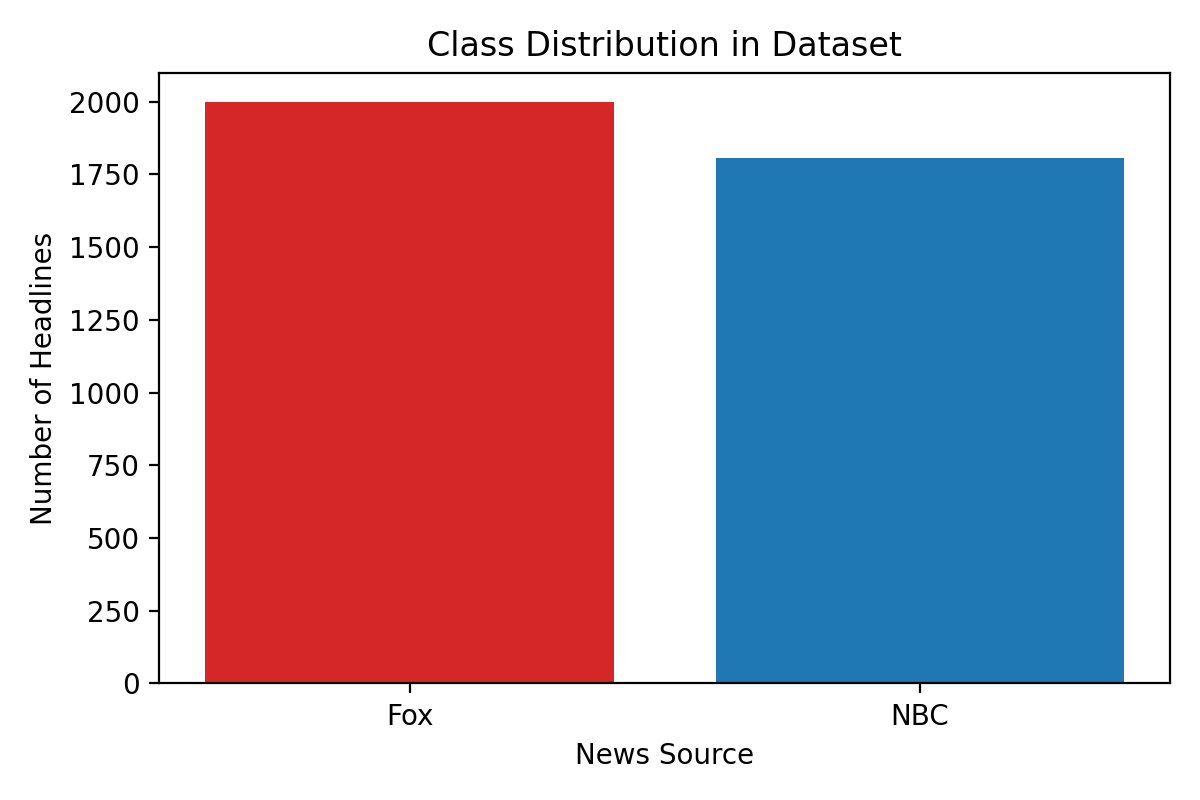
\includegraphics[width=\linewidth]{Figures/class_distribution.png}
\caption{Class balance after filtering to the two domains.}
\label{fig:class}
\end{subfigure}\hfill
\begin{subfigure}[t]{0.48\textwidth}
\centering
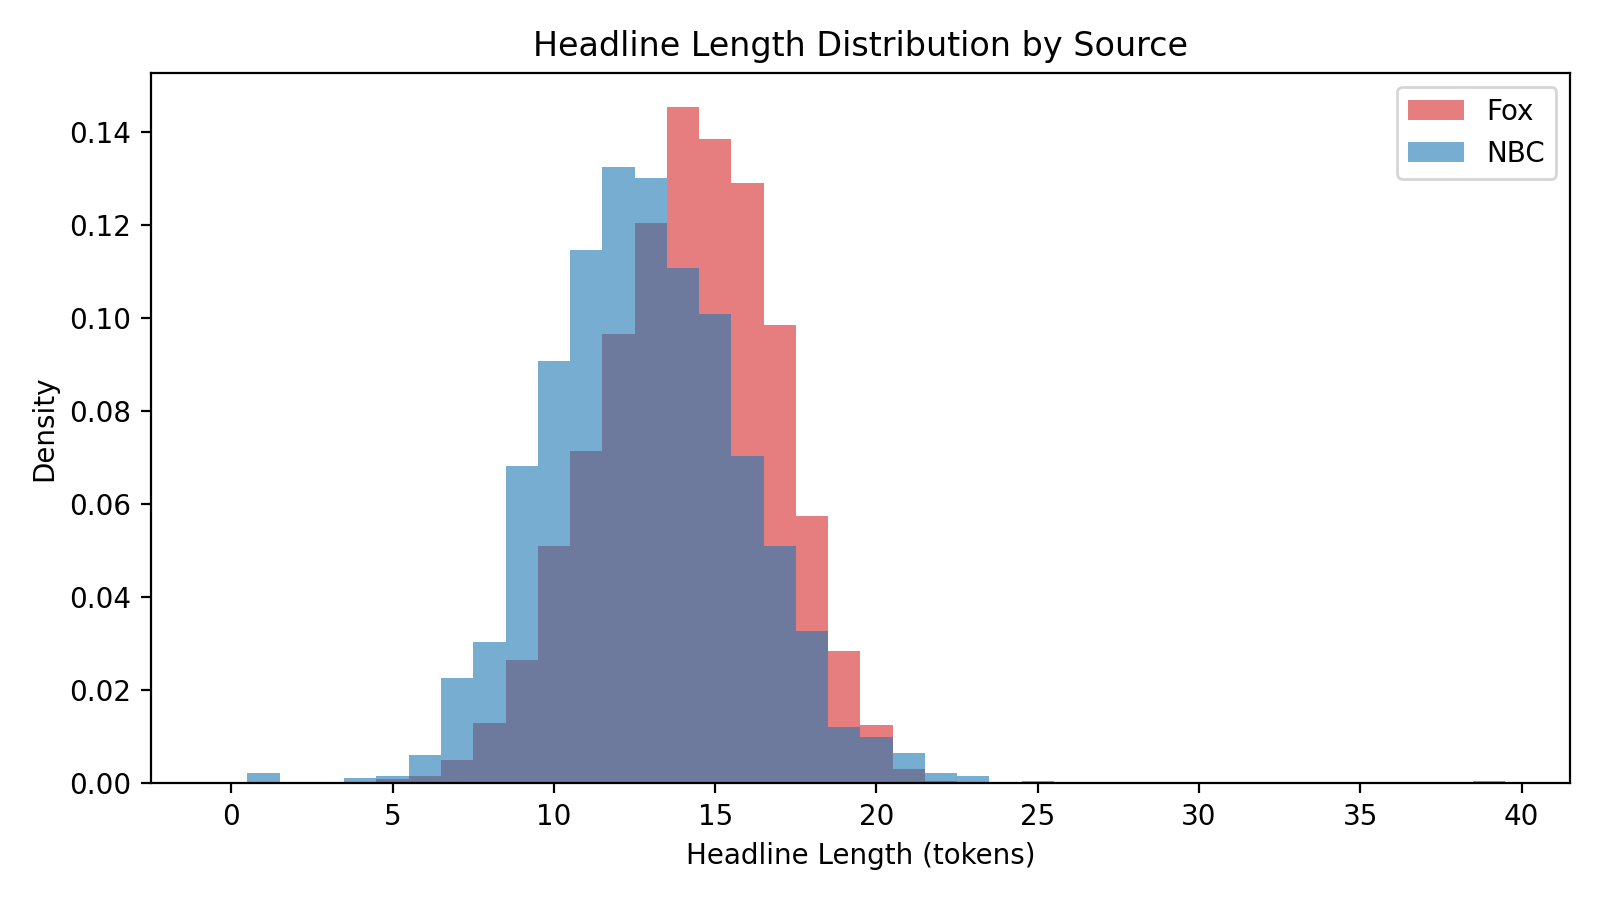
\includegraphics[width=\linewidth]{Figures/headline_length_distribution.png}
\caption{Headline length (characters).}
\label{fig:lengths}
\end{subfigure}
\caption{Dataset characteristics.}
\end{figure}

\begin{figure}[h]
\centering
\begin{subfigure}[t]{0.48\textwidth}
\centering
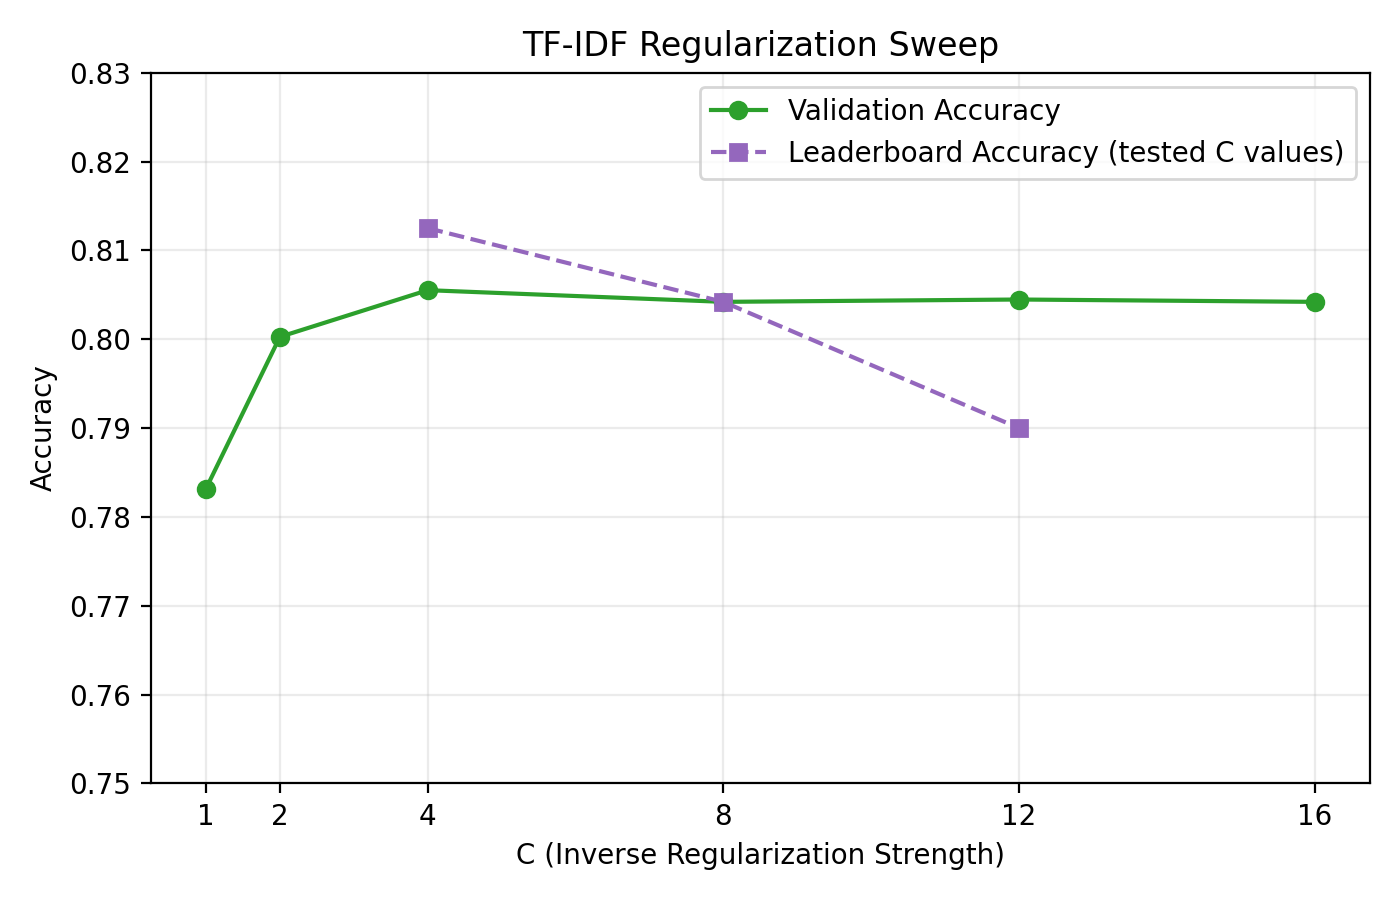
\includegraphics[width=\linewidth]{Figures/tfidf_c_sweep.png}
\caption{Regularisation sweep for the hashed TF-IDF logistic branch.}
\label{fig:csweep}
\end{subfigure}\hfill
\begin{subfigure}[t]{0.48\textwidth}
\centering
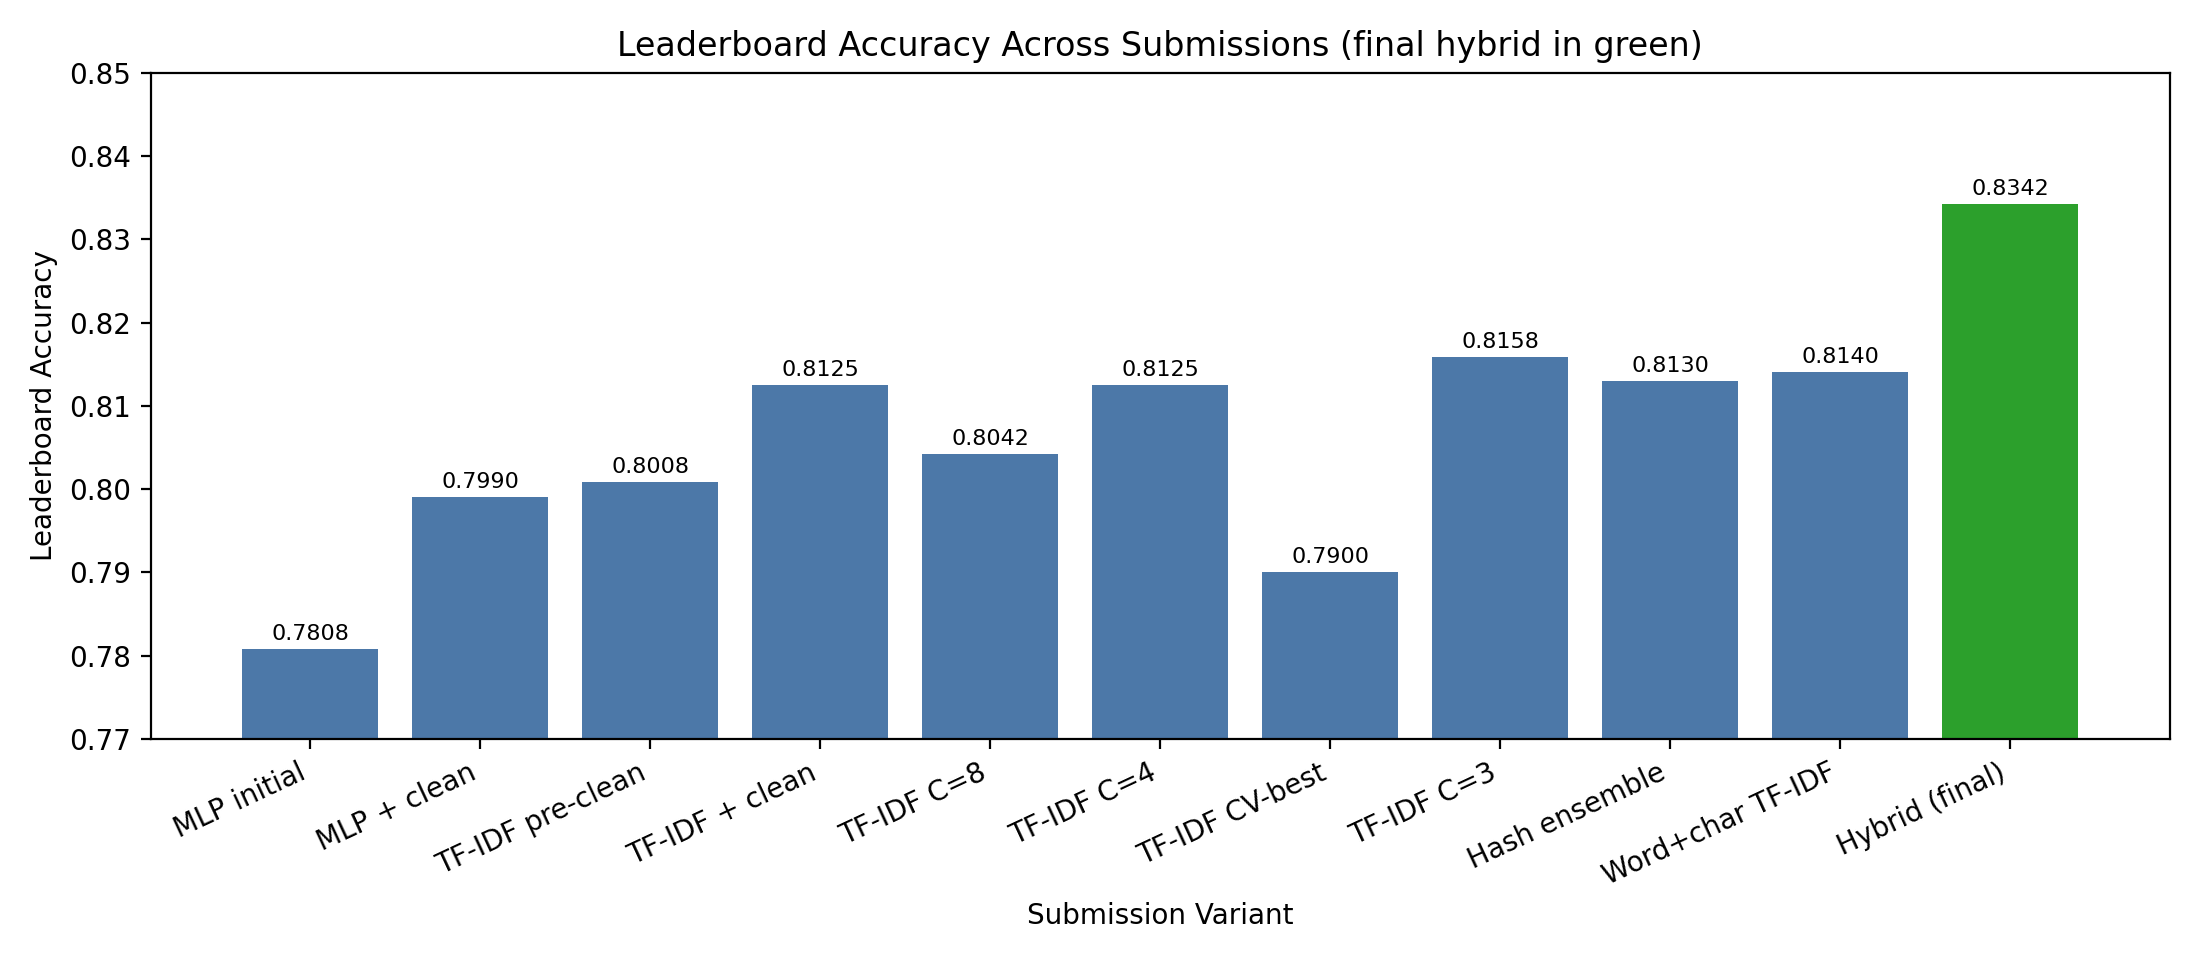
\includegraphics[width=\linewidth]{Figures/leaderboard_progression.png}
\caption{Leaderboard accuracy over time.}
\label{fig:lb}
\end{subfigure}
\caption{Tuning and submission timeline.}
\end{figure}

\begin{figure}[h]
\centering
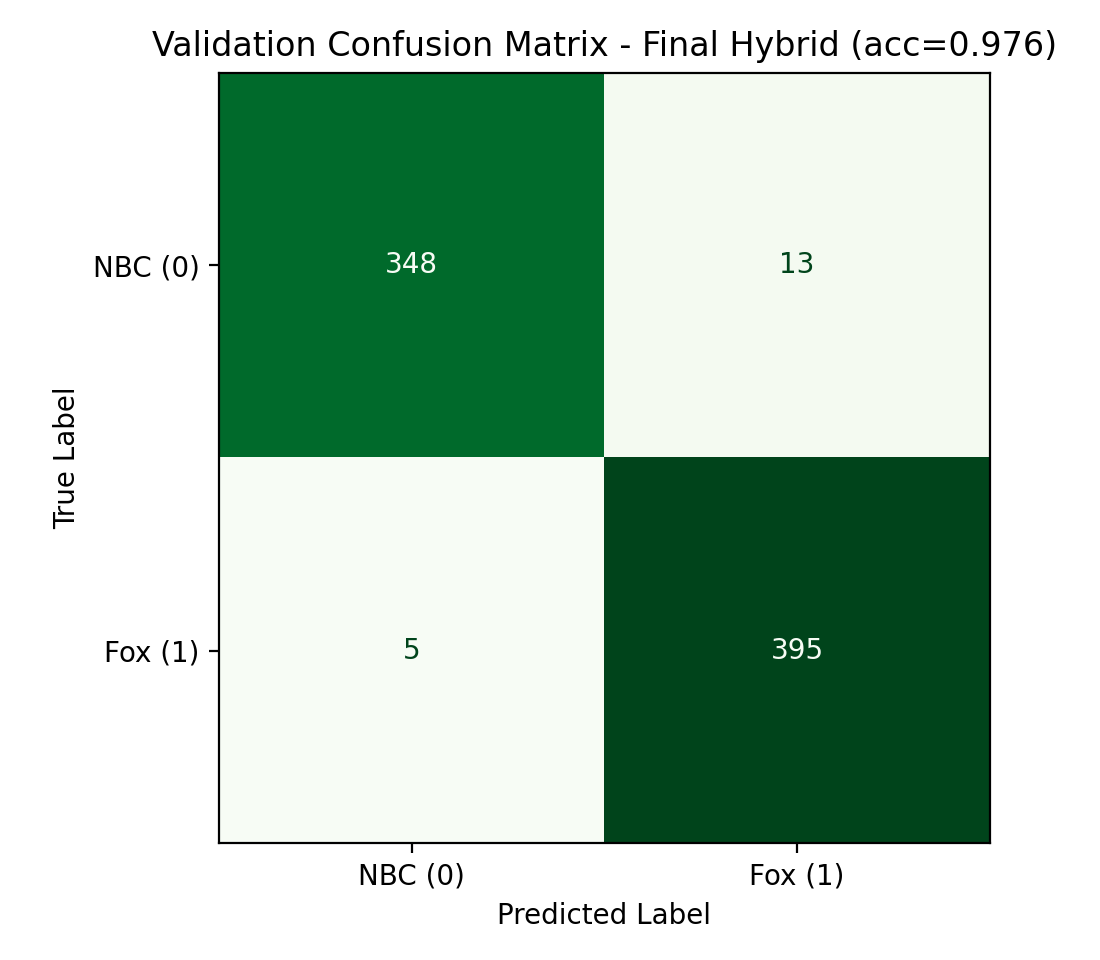
\includegraphics[width=0.55\linewidth]{Figures/validation_confusion_matrix_final_model.png}
\caption{Validation confusion matrix for the final hybrid model (\texttt{final\_model.pt}).}
\label{fig:cm}
\end{figure}

\begin{figure}[h]
\centering
\begin{subfigure}[t]{0.48\textwidth}
\centering
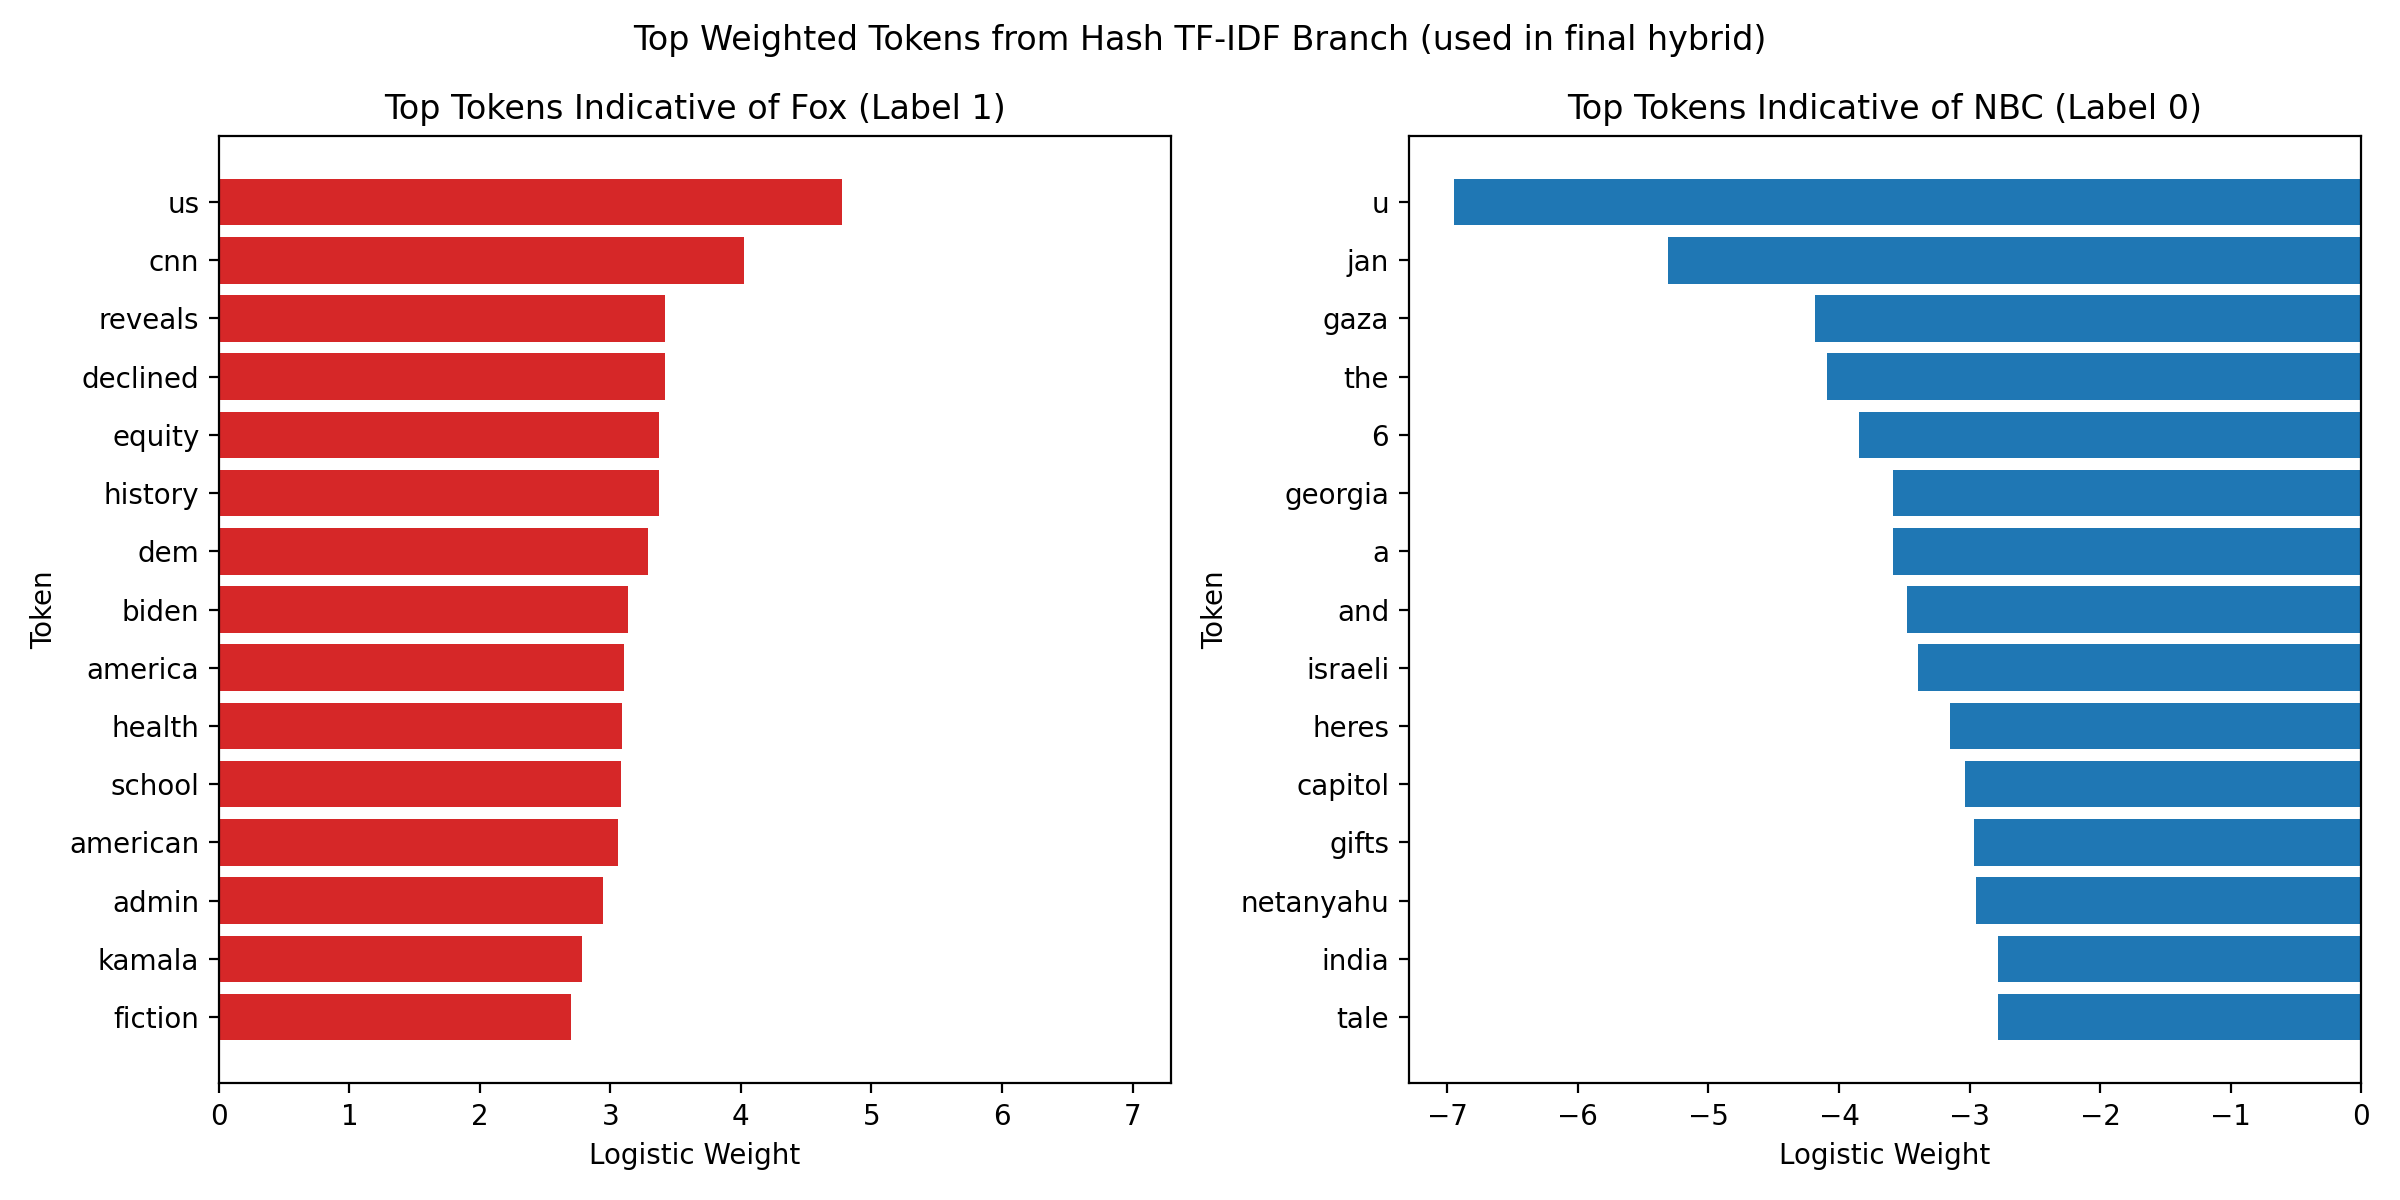
\includegraphics[width=\linewidth]{Figures/top_weighted_tokens_hash.png}
\caption{Hashed TF-IDF branch (\texttt{model\_tfidf\_c3.pt}).}
\label{fig:tokens-hash}
\end{subfigure}\hfill
\begin{subfigure}[t]{0.48\textwidth}
\centering
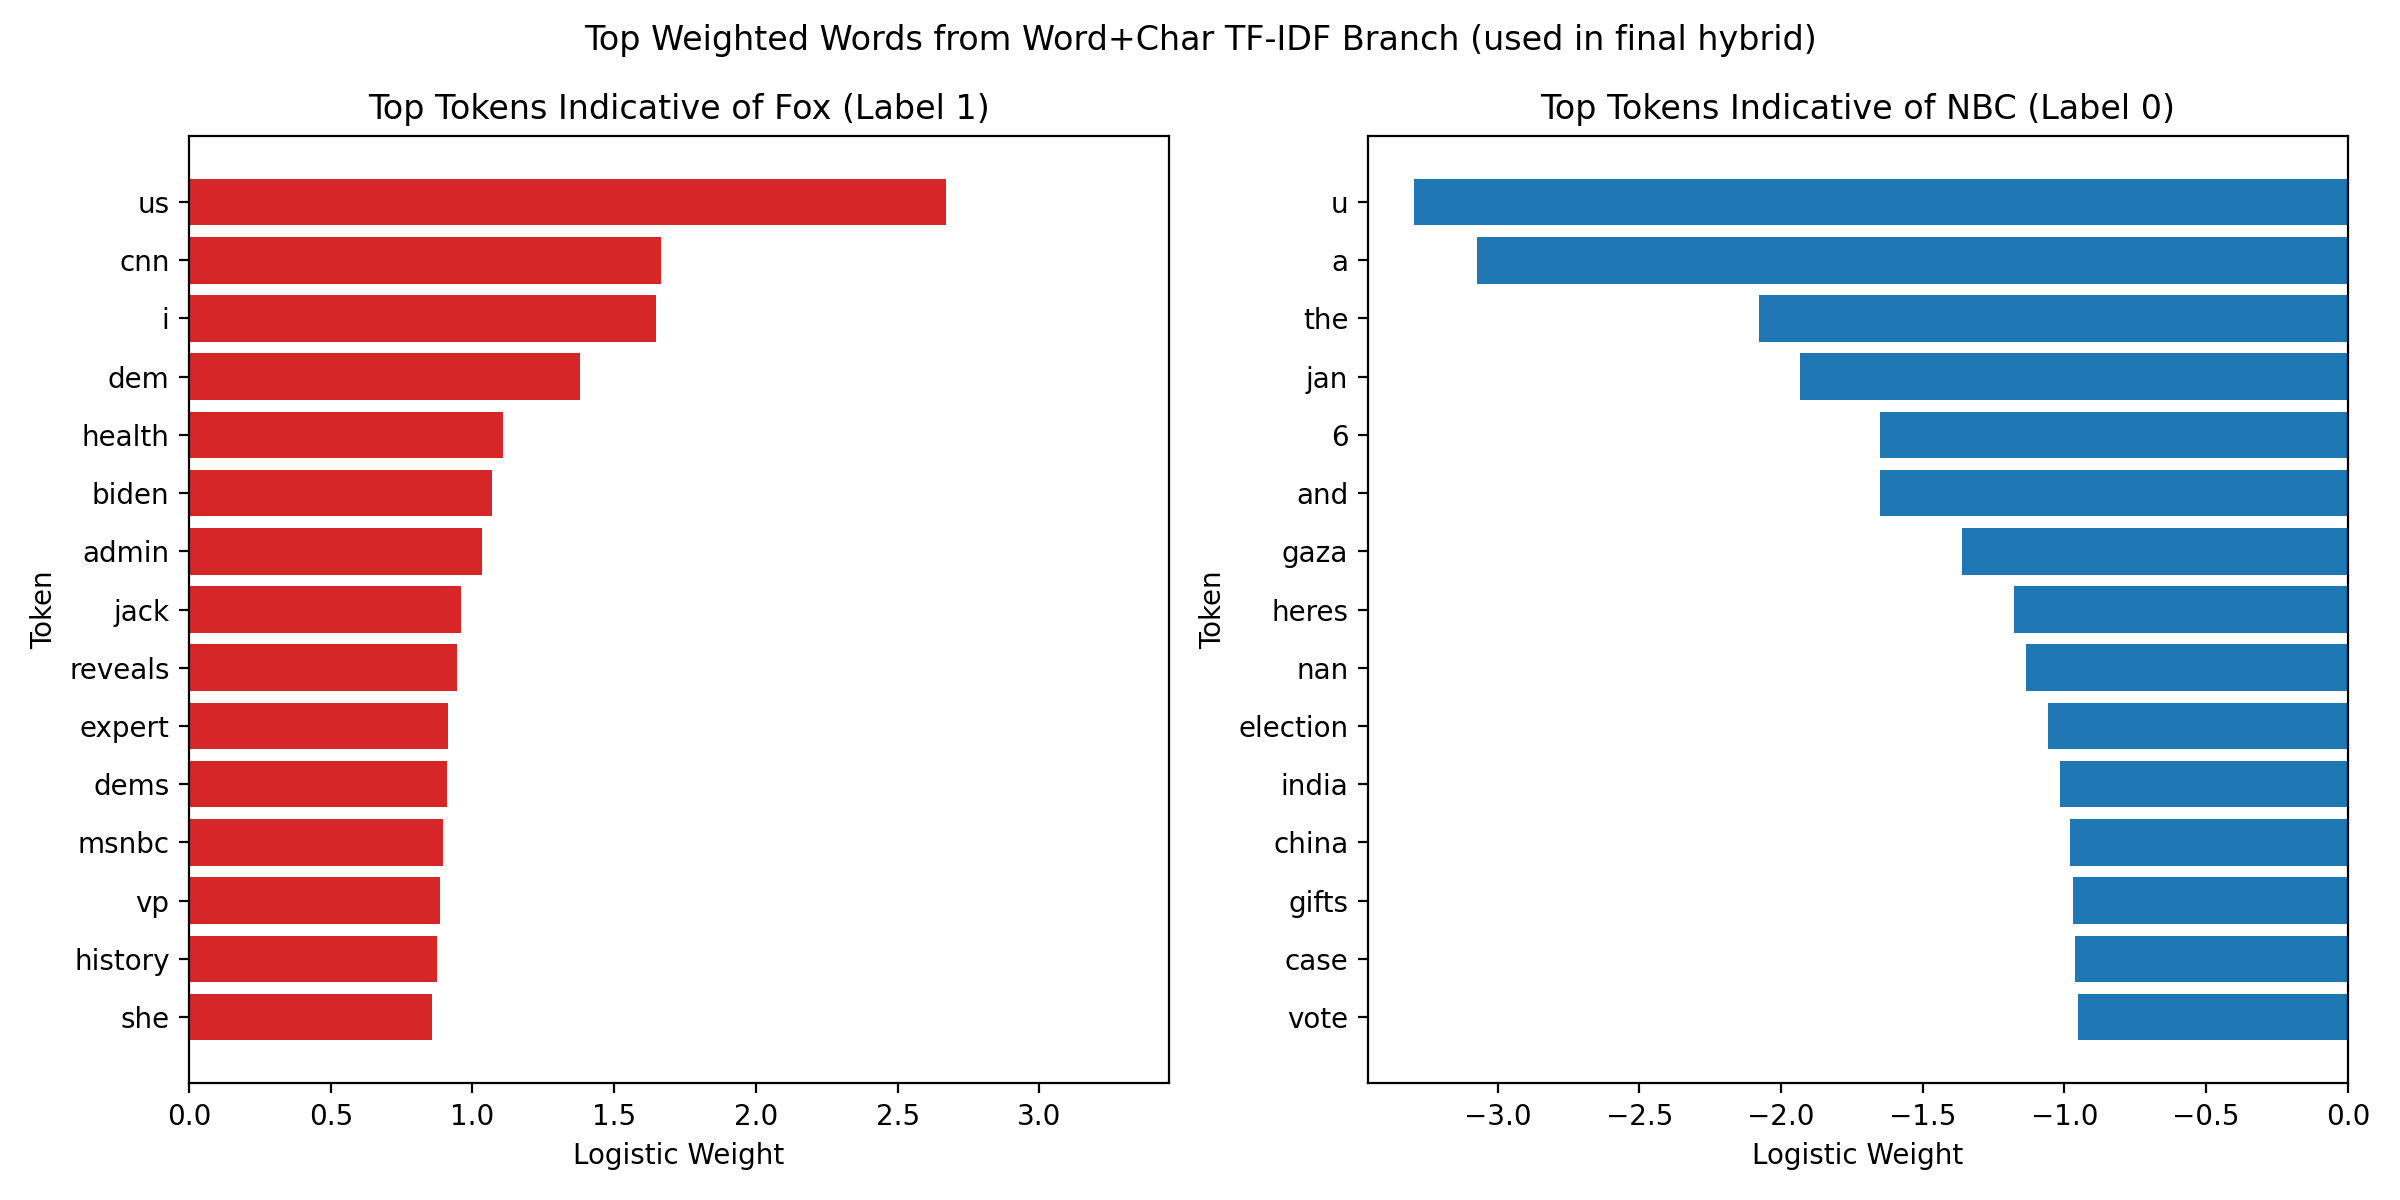
\includegraphics[width=\linewidth]{Figures/top_weighted_tokens_word_char.png}
\caption{Word+character TF-IDF branch (word part of \texttt{model\_vocab\_char\_c4.pt}).}
\label{fig:tokens-vocab}
\end{subfigure}
\caption{Most positively (Fox) and most negatively (NBC) weighted tokens in the two branches that compose the final hybrid model.}
\end{figure}

\newpage
\section{Exploratory Component}

For the exploratory component of the project, we wanted to collect and curate our own dataset on a new topic. Since we didn't get the chance to collect our own data for the news classification portion, along with the low dimensionality of the Fox vs. NBC data, we decided to collect and pre-process data relating to a topic of interest for our group: College Football.\\

As sports and technology have evolved in recent years, machine learning has become integral to how coaches, teams, leagues, and sports analysts understand and evaluate performance. With fairly accessible, high-quality datasets and new advancements in computational power, it’s now possible to investigate many complex questions about game strategy, team efficiency, and competitive outcomes across the world of sports. College football provides a rich environment for quantitative study due to its large number of features, diverse styles of play, and significant variability in team strength and performance from week to week. As a result, it has become quite an appealing domain for applying methods from statistics, data science, and machine learning.\\

Among the many facets of college football, \textit{one-score games} (matchups decided by a point differential of 8 or less) represent an interesting scenario. These games are defined by narrow margins in which small changes in team/individual performance can alter the final result. Unlike “blowouts”, where clear differences in talent typically dictate outcomes, one-score contests often hinge on subtle details such as turnover margin, total yards, third-down conversion rates, or time of possession. Understanding what differentiates winning and losing performances in these tight scenarios is valuable not only for predictive modeling but also for gaining insight into how teams respond under such high-pressure conditions. For these reasons, we decided to curate our dataset strictly on one-score college football games, over the last 10 years. We also chose to collect this past year's data as a hold-out test set to be used for model evaluation.\\

Our data collection involved crafting a dataset of the relevant team stats from all one-score FBS matchups\footnote{FBS is the highest level of collegiate football in the NCAA.} played from the years 2014 to 2025. Each game is labeled by a unique 9-digit ``game ID", which we simply retrieved from \href{collegefootballdata.com}{collegefootballdata.com} (CFBD). The CFBD website offers a free API key to directly query their database from a personal device. Using this method, we were able to again retrieve the game IDs, then use those to fetch the team statistics from all of the games. In total, this method retrieved data from 9,414 FBS games and included 43 features for each team (game ID, points, time of possession, etc.). See the Exploratory Component folder in our \href{https://github.com/HarounShah/cis5190-final-project}{GitHub repo} for the API querying. This method still had some missing data; however, it appeared to be the most complete option to allow us to conduct data pre-processing.

To carry out data pre-processing, we labeled each row with the label/class as follows:
\[ \begin{cases} 
      1 & \text{if home team won} \\
      0 & \text{if home team lost}
   \end{cases}
\]
Then, in a similar fashion, created a new feature that compares the home team's points to the away team's, and if the difference is less or equal to than 8, it is labeled as a one-score game:
\[ \begin{cases} 
      1 & \text{if }||\text{ home team score} - \text{away team score}|| \leq  8\\
      0 & \text{if otherwise}
   \end{cases}
\]

Any columns that could be deemed unimportant or were missing large amounts of data were removed. For example, the \textit{puntReturns} feature (the number of times a team receives a punt) had over 800 missing data points, and the feature itself may not be important enough to warrant the significant decrease in training data. Similar features included \textit{kickReturns} (the number of times a team receives a kick) and \textit{totalPenaltiesYards} (the number of penalties a team receives along with the amount of yards they are penalized). After selecting just the one-score games, the number of rows (games) decreased from 9,414 to 3,239. Additionally, after removing all rows with missing data, it decreased further to 2623 games. We are then left with two columns for each team statistic (eg., \textit{firstDowns\_home} and \textit{firstDowns\_away}). Using these features in machine learning models could be misleading and redundant. We are interested in exploring how these statistics contribute to a team \textit{winning} a game, which implies that the opposing team loses that same game. For example, even if the home team gets 20 first downs and the away team gets 27, then that should decrease the probability of any model to label this game as a win for the home team. In essence, the statistics are only indicative of a team's chances of winning when compared to the statistics of the opposing team. For this reason, a ``difference'' feature for each \_home and \_away pair is computed (eg. \textit{firstDowns\_diff} is defined as \textit{firstDowns\_home} - \textit{firstDowns\_away}). This produced data with 16 ``difference'' feature columns defined as follows:
\begin{itemize}
    \item possessionTime\_diff
    \item interceptions\_diff
    \item fumblesLost\_diff
    \item turnovers\_diff
    \item yardsPerRushAttempt\_diff
    \item rushingYards\_diff
    \item yardsPerPass\_diff
    \item netPassingYards\_diff
    \item totalYards\_diff
    \item firstDowns\_diff
    \item tacklesForLoss\_diff
    \item tackles\_diff
    \item sacks\_diff
    \item qbHurries\_diff
    \item passesDeflected\_diff
    \item thirdDown\%\_diff
\end{itemize}

By the end, we are left with two processed datasets: one containing team difference statistics from 2623 games in the years 2014-2024 to serve as training data, and another containing 312 games from the 2025 college football season to serve as the testing data. If used for modeling, different splitting techniques could be utilized, such as including a validation set, or using stratified/k-fold cross validation.

The balance of class labels is an important factor to consider before training models. Large class imbalances can lead to misleading results, ineffective models, and thus, more effort to subdue these issues. Across the 2623 one-score games in the training dataset, the home team won 1433 games ($54.63\%$), while the away team won 1190 games ($45.37\%$). Thus, the class distribution is only mildly imbalanced and does not require aggressive imbalance correction.

\begin{figure}[h!]
\centering
\includegraphics[scale = 0.4]{ClassBalance.png}
\caption{Class balance of one-score games in the training data.}
\label{fig:class_balance}
\end{figure}

It is important that we get a good understanding of all of our features. Firstly, we can observe the numerical summary of each feature. Table \ref{tab:five_number_summary} gives an initial idea of the range and spread of each feature. Most features have varying scales of magnitude, but all have a mean equal to or close to 0. This is to be expected, as any mean away from 0 would hint at some sort of home-field advantage/disadvantage. 

\begin{table}
\centering
\small
\begin{tabular}{lrrrrrrr}
\toprule
\textbf{Feature} & \textbf{Mean} & \textbf{Std} & \textbf{Min} & \textbf{25\%} & \textbf{50\%} & \textbf{75\%} & \textbf{Max} \\
\midrule
possessionTime\_diff      & -15.3019 & 539.5982 & -1762.0 & -370.0 &  -34.0 &  354.0 & 1936.0 \\
interceptions\_diff       &  -0.0206 &   1.2278 &    -5.0 &   -1.0 &    0.0 &    1.0 &    5.0 \\
fumblesLost\_diff         &   0.0271 &   1.0812 &    -4.0 &   -1.0 &    0.0 &    1.0 &    4.0 \\
turnovers\_diff           &   0.0065 &   1.5876 &    -6.0 &   -1.0 &    0.0 &    1.0 &    5.0 \\
yardsPerRushAttempt\_diff &   0.0396 &   2.0226 &    -7.3 &   -1.3 &    0.1 &    1.4 &    9.3 \\
rushingYards\_diff        &   3.0698 & 108.4108 &  -458.0 &   -67.0 &  4.0 &   75.5 &  394.0 \\
yardsPerPass\_diff        &   0.0618 &   2.9772 &   -19.0 &   -1.7 &    0.1 &    1.8 &   36.5 \\
netPassingYards\_diff     &  -1.6805 & 115.7711 &  -425.0 &   -79.0 &    0.0 &   78.0 &  402.0 \\
totalYards\_diff          &   1.3965 &  99.2184 &  -375.0 &   -66.0 &    4.0 &   68.0 &  328.0 \\
firstDowns\_diff          &   0.1704 &   6.6146 &   -21.0 &   -4.0 &    0.0 &    4.0 &   23.0 \\
tacklesForLoss\_diff      &   0.0660 &   3.7975 &   -26.0 &   -2.0 &    0.0 &    3.0 &   25.0 \\
tackles\_diff             &  -1.1144 &  14.0380 &   -91.0 &   -9.0 &   -1.0 &    7.0 &   86.0 \\
sacks\_diff               &   0.1254 &   2.4958 &   -12.0 &   -1.0 &    0.0 &    2.0 &   18.0 \\
qbHurries\_diff           &   0.6901 &   2.8980 &   -15.0 &   -1.0 &    0.0 &    2.0 &   19.0 \\
passesDeflected\_diff     &   0.4258 &   3.3046 &   -18.0 &   -2.0 &    0.0 &    2.0 &   16.0 \\
thirdDown\%\_diff         &   0.0006 &   0.1660 &   -0.6  &   -0.1 &    0.0 &    0.1 &   0.6 \\
\bottomrule
\end{tabular}
\caption{Five-number summaries and descriptive statistics for all numerical features.}
\label{tab:five_number_summary}
\end{table}

\newpage
What has been done here is only a brief start into the exploratory data analysis that can be done on our custom curated dataset. In the future, we hope to use this data to train models and better understand the driving factors of winning close matchups at the highest level of collegiate football.

\end{document}
